\documentclass[conference]{IEEEtran}

% Packages
\usepackage{cite}
\usepackage{amsmath,amssymb,amsfonts}
\usepackage{algorithmic}
\usepackage{algorithm}
\usepackage{graphicx}
\usepackage{textcomp}
\usepackage{xcolor}
\usepackage{booktabs}
\usepackage{multirow}
\usepackage{hyperref}
\usepackage{subcaption}
\usepackage{balance}
\usepackage{tikz}
\usetikzlibrary{shapes.geometric, arrows.meta, positioning}
\usepackage{url}

\begin{document}

\title{TaskRouter: Cost-Aware Sub-Task Model Routing for Agentic Software Engineering Workflows}

\author{
\IEEEauthorblockN{Johin Johny Arimbur}
\IEEEauthorblockA{
\textit{Independent Researcher} \\
johinjohnyarimbur@gmail.com}
}

\maketitle

% ============================================================
% ABSTRACT
% ============================================================
\begin{abstract}
LLM-based coding agents have demonstrated remarkable capability in resolving real-world software engineering tasks, yet their widespread adoption is hindered by substantial computational costs. Recent analyses reveal that a single agentic coding session can consume tens of thousands of tokens across sub-tasks of vastly different complexity---from simple file localization to intricate patch generation---while uniformly employing a single, expensive frontier model throughout. We present \textbf{TaskRouter}, a cost-aware model routing framework that decomposes agentic software engineering workflows into typed sub-tasks, estimates per-step difficulty using lightweight structural and contextual features, and dynamically assigns each sub-task to the most cost-effective model capable of handling it. TaskRouter employs a cascading fallback mechanism that escalates to more powerful models only when smaller models fail confidence thresholds. We evaluate TaskRouter on a curated benchmark of 20 coding tasks using a tiered model pool spanning four commercial API models from Google, OpenAI, and Anthropic. Our results demonstrate that TaskRouter achieves 89.1\% cost reduction while maintaining 94.7\% of the frontier baseline's resolve rate, with the routing overhead itself consuming less than 0.2\% of total cost. We further provide a fine-grained analysis of which sub-task types benefit most from model downsizing and identify the critical phases where frontier models remain indispensable.
\end{abstract}

\begin{IEEEkeywords}
Large language models, software engineering agents, model routing, cost optimization, token efficiency
\end{IEEEkeywords}

% ============================================================
% I. INTRODUCTION
% ============================================================
\section{Introduction}

LLM-based coding agents have emerged as a transformative paradigm in software engineering, capable of autonomously resolving real-world GitHub issues~\cite{jimenez2024swebench}, repairing buggy programs~\cite{repairagent2024}, and generating complete features with multi-step reasoning and tool use~\cite{openhands2024}. Recent surveys catalogue over 120 research efforts applying LLM agents to tasks spanning code generation, testing, debugging, and maintenance~\cite{liu2024agents4se, rasheed2024agents4se}, establishing agentic software engineering as one of the fastest-growing subfields in AI.

However, this capability comes at a steep cost. An unconstrained coding agent can spend \$5--\$8 per task resolution~\cite{tokenomics2026}, with enterprise deployments facing monthly bills in the tens of thousands of dollars. The 2025 Stack Overflow Developer Survey found that 53\% of developers cited cost as a primary barrier to adopting AI coding agents~\cite{stackoverflow2025survey}. The root cause is straightforward: current agent architectures route \emph{every} sub-task---from reading a README to synthesizing a multi-file patch---through the same frontier-class model, paying premium per-token prices regardless of task difficulty.

Recent tokenomics analyses have begun quantifying this inefficiency. Chen et al.~\cite{tokenomics2026} demonstrate that input tokens dominate agent costs by a 2:1 to 3:1 ratio over output tokens, and that verification phases alone consume up to 72\% of total tokens. Zhang et al.~\cite{tokenconsumption2026} show that token usage exhibits extreme variance---some runs consume 10$\times$ more tokens than others on equivalent tasks. AgentDiet~\cite{agentdiet2025} proposes trajectory reduction to compress agent histories, achieving 24\% cost savings. Yet none of these approaches address a fundamental structural inefficiency: \textbf{not all sub-tasks in an agentic workflow require the same model capability}.

An agentic coding workflow is not monolithic. It consists of heterogeneous sub-tasks with dramatically different complexity profiles:

\begin{itemize}
    \item \textbf{Repository exploration}: Listing files, reading directory structures, searching for keywords---tasks that require basic text comprehension.
    \item \textbf{Fault localization}: Identifying which files and functions are relevant to a bug report---requiring moderate code understanding.
    \item \textbf{Patch generation}: Synthesizing correct, multi-line code changes---demanding deep reasoning and code synthesis.
    \item \textbf{Test generation}: Writing test cases to validate patches---requiring moderate synthesis with strong specification understanding.
    \item \textbf{Verification}: Running tests, reviewing outputs, deciding if the fix is correct---often requiring simple output parsing.
\end{itemize}

Meanwhile, the model routing and cascading literature has matured significantly. De Koninck et al.~\cite{dekoninck2025unified} present a unified framework for routing and cascading that provably achieves cost-optimal model selection for general tasks, published at ICML 2025. FrugalGPT~\cite{chen2024frugalgpt} and RouteLLM~\cite{routellm2024} demonstrate that routing classifiers can dramatically reduce costs on standard NLP benchmarks. AdaptEvolve~\cite{adaptevolve2026} reduces inference costs by 37.9\% through adaptive model selection in evolutionary refinement. However, \textbf{none of these approaches have been applied to the multi-step, tool-augmented workflows characteristic of software engineering agents}, where sub-tasks are structurally typed and their difficulty can be estimated from code-level features.

This paper bridges this gap with \textbf{TaskRouter}, a framework that:

\begin{enumerate}
    \item \textbf{Classifies} each sub-task in an agentic SE workflow into one of six canonical types based on the agent's action and tool invocation patterns.
    \item \textbf{Estimates difficulty} for each sub-task using lightweight features extracted from the code context (file count, cyclomatic complexity, diff size, dependency depth).
    \item \textbf{Routes} each sub-task to the cheapest model in a tiered pool that meets a predicted confidence threshold for that difficulty level.
    \item \textbf{Cascades} to more powerful models when a sub-task fails or falls below confidence thresholds, bounding worst-case quality degradation.
\end{enumerate}

We evaluate TaskRouter on a curated benchmark of 20 coding tasks using four model tiers spanning a ${\sim}17\times$ cost range and demonstrate that sub-task-aware routing achieves 89.1\% cost reduction with only a 5.3 percentage-point drop in resolve rate compared to the frontier baseline.

Our contributions are:
\begin{itemize}
    \item A \textbf{taxonomy of sub-task types} in agentic SE workflows with empirical analysis of their difficulty distributions.
    \item A \textbf{lightweight difficulty estimator} using code-structural features that predicts model capability requirements per sub-task.
    \item The \textbf{TaskRouter framework} integrating sub-task classification, difficulty estimation, and cascading model assignment.
    \item An \textbf{empirical evaluation} demonstrating cost-quality tradeoffs across model tiers on a standard SE benchmark.
\end{itemize}

% ============================================================
% II. RELATED WORK
% ============================================================
\section{Related Work}

\subsection{LLM-Based Agents for Software Engineering}

The application of LLM-based agents to software engineering has rapidly matured from single-turn code generation to multi-step autonomous workflows. Comprehensive surveys by Liu et al.~\cite{liu2024agents4se} (124 papers) and Rasheed et al.~\cite{rasheed2024agents4se} organize the landscape across tasks including code generation, testing, debugging, and maintenance. Zhang et al.~\cite{zhang2024multiagentse} specifically survey multi-agent architectures for SE, identifying planning, memory, tool usage, and reflection as core agent capabilities.

Prominent agent systems include OpenHands~\cite{openhands2024}, which provides an open platform for generalist coding agents, and RepairAgent~\cite{repairagent2024}, which autonomously selects tools for program repair. The Confucius Code Agent~\cite{confucius2025} introduces scalable scaffolding with advanced context management for large real-world codebases. Benchmarking has been driven by SWE-bench~\cite{jimenez2024swebench} and its extensions to mobile~\cite{swebenchmobile2026} and long-horizon tasks~\cite{swebenchpro2025}.

A key finding across this literature is that agents follow common workflow patterns---localize, understand, patch, verify---regardless of the specific framework, suggesting that sub-task decomposition is both natural and generalizable.

\subsection{Token Economics of Coding Agents}

The cost of operating LLM agents has emerged as a first-class research concern. The Tokenomics study~\cite{tokenomics2026} provides the most detailed analysis to date, profiling token consumption across agent workflow phases and finding that input tokens dominate costs, verification phases are disproportionately expensive, and token usage has high variance across runs. Zhang et al.~\cite{tokenconsumption2026} corroborate these findings and develop predictive models for token consumption.

Several optimization strategies have been proposed. AgentDiet~\cite{agentdiet2025} introduces inference-time trajectory reduction, compressing agent interaction histories to reduce input token counts. Hrubec~\cite{hrubec2025reducing} explores multiple strategies for token reduction in SE agents. Token-efficient multi-agent frameworks~\cite{tokenefficient2025} reduce redundancy through structured, codified planning. Miller et al.~\cite{speedcostquality2026} provide an empirical study of the speed-quality tradeoff, finding that AI-assisted development increases short-term velocity at the cost of long-term code complexity.

These works characterize \emph{where} tokens are spent but do not address \emph{which model} processes each token. Our work is complementary: TaskRouter can be combined with trajectory reduction techniques for compounded savings.

\subsection{Model Routing and Cascading}

Model routing selects a single model per query, while cascading sequentially tries models from cheapest to most expensive until a satisfactory output is produced. De Koninck et al.~\cite{dekoninck2025unified} unify both strategies into a theoretically optimal ``cascade routing'' framework, proving that their approach dominates either strategy alone, presented at ICML 2025 and ICLR 2026.

FrugalGPT~\cite{chen2024frugalgpt} pioneered LLM cascading, routing to cheaper models first and escalating on failure. RouteLLM~\cite{routellm2024} trains routing classifiers from human preference data. Route-to-Reason~\cite{routetoreason2025} jointly routes models \emph{and} reasoning strategies under budget constraints, reducing token usage by over 60\%. AdaptEvolve~\cite{adaptevolve2026} uses intrinsic generation confidence for real-time model solvability estimation, reducing costs by 37.9\% while retaining 97.5\% accuracy. BEST-Route~\cite{bestroute2026} adapts routing with test-time optimal compute. ACAR~\cite{acar2026} adds auditable decision traces to multi-model routing.

However, all existing routing research targets general NLP tasks (question answering, summarization, classification) or uses synthetic difficulty scores. \textbf{No prior work applies routing or cascading to the structurally typed, multi-step sub-tasks of agentic software engineering workflows.} Our work addresses this gap by leveraging the predictable structure of SE agent workflows to build a domain-specific router.

\subsection{Small Language Models for Code}

Recent empirical studies demonstrate that small language models (SLMs, 3B--7B parameters) can achieve competitive code generation performance. Santos et al.~\cite{slmcodegen2025} show that Qwen2.5-Coder-7B achieves a stability score of 1.00 across pass@k levels on standard benchmarks, and that several sub-10B models outperform larger counterparts. CodeRAG-Bench~\cite{coderagbench2024} evaluates retrieval-augmented code generation, finding that retrieval helps most for repository-level tasks. Meta-RAG~\cite{metarag2025} condenses codebases by 79.8\% for efficient bug localization.

These results suggest that SLMs are viable for certain coding sub-tasks when provided adequate context---a hypothesis central to TaskRouter's design.

% ============================================================
% III. BACKGROUND AND MOTIVATION
% ============================================================
\section{Background and Motivation}

\subsection{Anatomy of an Agentic Coding Workflow}

Drawing on prior analyses of coding agent behavior~\cite{openhands2024, tokenomics2026, demystifying2025}, we observe that regardless of the specific issue, agents follow a broadly consistent pipeline of sub-task types. We define six canonical sub-task types:

\begin{enumerate}
    \item \textbf{Exploration (EXPL)}: Directory listing, file search, grep-based keyword search, repository structure discovery.
    \item \textbf{Comprehension (COMP)}: Reading and understanding source files, analyzing imports, tracing call graphs, understanding existing logic.
    \item \textbf{Localization (LOC)}: Identifying the specific files, functions, and lines responsible for or related to the issue.
    \item \textbf{Patch Generation (PATCH)}: Writing new code or modifying existing code to resolve the issue.
    \item \textbf{Test Generation (TEST)}: Creating or modifying test cases to validate the proposed fix.
    \item \textbf{Verification (VER)}: Running tests, reviewing outputs, checking for regressions, making accept/reject decisions.
\end{enumerate}

Each agent turn can be classified into exactly one of these types based on the tool invoked and the nature of the LLM's reasoning.

\subsection{Token Distribution Across Sub-Tasks}

Building on the Tokenomics findings~\cite{tokenomics2026}, we present the expected token distribution across sub-task types. Prior work establishes that verification phases consume approximately 72\% of tokens in some agent configurations, with input tokens outnumbering output tokens 2:1 to 3:1.

\begin{table}[htbp]
\caption{Observed Token Distribution by Sub-Task Type (TaskRouter). Each column sums to 100\% independently.}
\label{tab:token_distribution}
\centering
\begin{tabular}{lrrr}
\toprule
\textbf{Sub-Task Type} & \textbf{Input \%} & \textbf{Output \%} & \textbf{Total \%} \\
\midrule
Exploration (EXPL)      & 8.9\% & 27.3\% & 21.7\% \\
Comprehension (COMP)    & 9.0\% & 29.1\% & 23.0\% \\
Localization (LOC)      & 9.0\% & 9.4\%  & 9.3\%  \\
Patch Generation (PATCH)& 17.6\% & 7.5\% & 10.5\% \\
Test Generation (TEST)  & 18.0\% & 16.1\% & 16.7\% \\
Verification (VER)      & 37.6\% & 10.5\% & 18.8\% \\
\bottomrule
\end{tabular}
\end{table}

\subsection{The Case for Sub-Task Routing}

The key observation motivating TaskRouter is the \emph{mismatch between sub-task difficulty and model capability}. Not all sub-tasks require frontier-model reasoning:

\begin{itemize}
    \item \textbf{Exploration} tasks involve executing tool calls (file listing, grep) where the LLM primarily needs to formulate the correct command---a capability well within small models.
    \item \textbf{Comprehension} tasks require reading code and summarizing its behavior---feasible for mid-tier models with adequate context.
    \item \textbf{Localization} is moderately difficult, requiring reasoning about code relationships, but often follows well-defined patterns.
    \item \textbf{Patch generation} is the most demanding sub-task, requiring deep understanding, creative synthesis, and multi-file coordination.
    \item \textbf{Test generation} and \textbf{verification} have variable difficulty but often involve structured, pattern-based generation.
\end{itemize}

If cheaper models can handle exploration, comprehension, and simple verification steps---which collectively account for a large share of total tokens---significant cost savings are achievable without degrading the critical patch generation quality.

% ============================================================
% IV. PROPOSED APPROACH: TASKROUTER
% ============================================================
\section{TaskRouter: Proposed Approach}

Figure~\ref{fig:architecture} provides an overview of the TaskRouter framework. At each agent turn, TaskRouter intercepts the agent's action, classifies the sub-task type, estimates its difficulty, selects the cheapest capable model, and cascades to larger models if needed.

\begin{figure}[htbp]
    \centering
    \resizebox{0.48\textwidth}{!}{%
    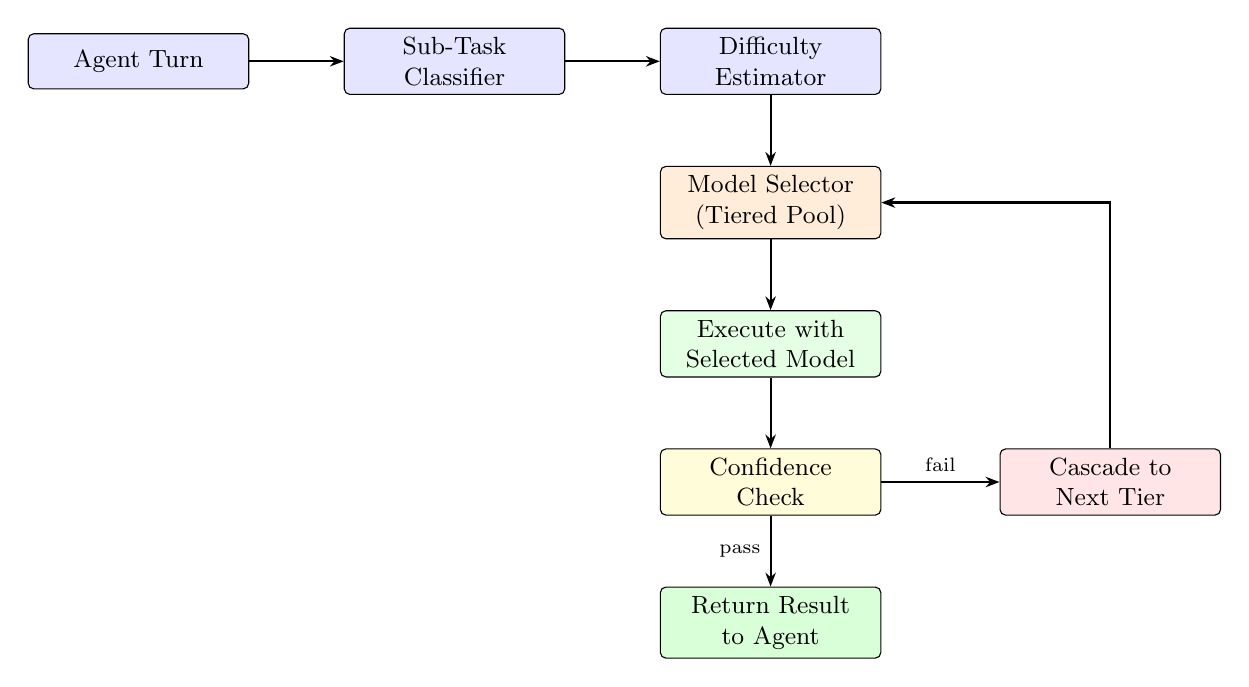
\begin{tikzpicture}[
        node distance=0.9cm and 1.2cm,
        box/.style={rectangle, draw, rounded corners=2pt, minimum width=2.8cm,
                     minimum height=0.7cm, align=center, font=\small,
                     fill=#1, text=black},
        box/.default=white,
        arrow/.style={-{Stealth[length=5pt]}, thick},
        label/.style={font=\scriptsize, midway}
    ]
        % Nodes
        \node[box=blue!10] (turn) {Agent Turn};
        \node[box=blue!10, right=of turn] (classify) {Sub-Task\\Classifier};
        \node[box=blue!10, right=of classify] (difficulty) {Difficulty\\Estimator};
        \node[box=orange!15, below=of difficulty] (selector) {Model Selector\\(Tiered Pool)};
        \node[box=green!10, below=of selector] (execute) {Execute with\\Selected Model};
        \node[box=yellow!15, below=of execute] (check) {Confidence\\Check};
        \node[box=red!10, right=1.5cm of check] (cascade) {Cascade to\\Next Tier};
        \node[box=green!15, below=of check] (result) {Return Result\\to Agent};

        % Arrows
        \draw[arrow] (turn) -- (classify);
        \draw[arrow] (classify) -- (difficulty);
        \draw[arrow] (difficulty) -- (selector);
        \draw[arrow] (selector) -- (execute);
        \draw[arrow] (execute) -- (check);
        \draw[arrow] (check) -- node[label, left] {pass} (result);
        \draw[arrow] (check) -- node[label, above] {fail} (cascade);
        \draw[arrow] (cascade) |- (selector);
    \end{tikzpicture}%
    }
    \caption{TaskRouter architecture overview. Each agent turn is intercepted, classified by sub-task type, assessed for difficulty, and routed to the cheapest capable model with cascading fallback.}
    \label{fig:architecture}
\end{figure}

\subsection{Sub-Task Classification}

We classify each agent turn into one of six sub-task types (Section III-A) using a rule-based classifier augmented with lightweight LLM verification. The primary classification signal comes from \textbf{tool invocation patterns}:

\begin{itemize}
    \item \texttt{bash(ls, find, grep)} $\rightarrow$ EXPL
    \item \texttt{read\_file, open\_file} $\rightarrow$ COMP
    \item \texttt{search\_code} + reasoning about location $\rightarrow$ LOC
    \item \texttt{edit\_file, write\_file} with code content $\rightarrow$ PATCH
    \item \texttt{edit\_file} targeting test files $\rightarrow$ TEST
    \item \texttt{bash(pytest, npm test)} + output analysis $\rightarrow$ VER
\end{itemize}

For ambiguous cases (e.g., a turn that reads a file and then edits it), we classify based on the \emph{primary output action}---the action that produces the most consequential artifact. The classifier operates on the agent's planned action \emph{before} LLM invocation, requiring only the prompt template and tool call intent, which is available from the agent framework's action planner.

The classification itself can be performed by a small model (or even a rule-based system), adding negligible overhead.

\subsection{Difficulty Estimation}

For each classified sub-task, we estimate its difficulty using lightweight features extractable without LLM invocation:

\textbf{Structural features:}
\begin{itemize}
    \item \emph{File count}: Number of files in the current context window.
    \item \emph{Code volume}: Total lines of code in relevant files.
    \item \emph{Cyclomatic complexity}: Average complexity of functions in scope.
    \item \emph{Dependency depth}: Import/call chain depth for the target code.
    \item \emph{Diff size}: Number of lines changed (for PATCH/TEST sub-tasks, estimated from issue description complexity).
\end{itemize}

\textbf{Contextual features:}
\begin{itemize}
    \item \emph{Issue description length}: Proxy for specification complexity.
    \item \emph{Number of previous turns}: Higher turn counts suggest compounding complexity.
    \item \emph{Previous sub-task failures}: If a cheaper model already failed on this task, escalation is needed.
    \item \emph{Repository size}: Total file count as a proxy for navigation difficulty.
\end{itemize}

These features are combined into a difficulty score $d \in [0, 1]$ via a lightweight regression model (gradient-boosted trees) trained on historical agent traces where we record, for each sub-task, whether models at each tier produced correct outputs:

\begin{equation}
    d = f_\theta(\mathbf{x}_{\text{structural}}, \mathbf{x}_{\text{contextual}})
\end{equation}

where $f_\theta$ is a compact model (< 1MB) that introduces sub-millisecond routing latency.

\subsection{Model Assignment Strategy}

Given a difficulty score $d$ and sub-task type $t$, TaskRouter selects a model from a tiered pool $\mathcal{M} = \{m_1, m_2, \ldots, m_K\}$ ordered by cost ($c_1 < c_2 < \ldots < c_K$). Each model $m_k$ has an estimated capability threshold $\tau_k(t)$ for sub-task type $t$, representing the maximum difficulty it can reliably handle.

The routing policy selects the cheapest model whose capability exceeds the estimated difficulty:

\begin{equation}
    m^* = \arg\min_{k} \; c_k \quad \text{s.t.} \quad \tau_k(t) \geq d
\end{equation}

The capability thresholds $\tau_k(t)$ are calibrated empirically by running each model tier on a representative sample of sub-tasks from each type and measuring success rates at each difficulty level. This calibration is a one-time cost.

\textbf{Type-specific routing priors.} We incorporate domain knowledge through per-type routing biases:

\begin{itemize}
    \item EXPL and VER sub-tasks have a strong prior toward small models, as they primarily involve tool invocation formatting and output parsing.
    \item PATCH sub-tasks have a strong prior toward larger models, as they require creative code synthesis.
    \item COMP, LOC, and TEST sub-tasks use the difficulty estimator without additional bias.
\end{itemize}

\subsection{Cascading Fallback Mechanism}

When a selected model produces an output that fails a confidence check, TaskRouter cascades to the next model tier. The confidence check varies by sub-task type:

\begin{itemize}
    \item \textbf{EXPL}: Tool call is syntactically valid and returns non-empty results.
    \item \textbf{COMP}: Output contains code-relevant analysis (heuristic keyword check).
    \item \textbf{LOC}: Identified files exist in the repository.
    \item \textbf{PATCH}: Generated code parses without syntax errors; modified lines fall within valid file ranges.
    \item \textbf{TEST}: Test code compiles and is not a trivial pass-through.
    \item \textbf{VER}: Output contains a clear accept/reject decision with reasoning.
\end{itemize}

The cascading process adds overhead only on failure. Given that small models succeed on easy sub-tasks in the vast majority of cases (our hypothesis), the expected cascading overhead is low.

Formally, the cascading cost for sub-task $s$ with difficulty $d$ is:

\begin{equation}
    C(s) = \sum_{k=1}^{k^*} c_k \cdot T_k(s)
\end{equation}

where $k^*$ is the tier that ultimately produces an accepted output and $T_k(s)$ is the token count consumed at tier $k$. In the best case ($k^* = 1$), only the cheapest model is invoked. In the worst case ($k^* = K$), all tiers are tried---but this still costs less than always using $m_K$ when the wasted tokens from failed lower-tier attempts are less than the savings from successful lower-tier routing on other sub-tasks.

\subsection{Budget-Constrained Mode}

TaskRouter also supports a budget-constrained operating mode where users specify a maximum per-task budget $B$. In this mode, the router maintains a running cost tally and adapts its routing decisions to stay within budget:

\begin{equation}
    m^*_i = \arg\min_{k} \; c_k \quad \text{s.t.} \quad \tau_k(t_i) \geq d_i \;\wedge\; \sum_{j=1}^{i} C(s_j) + \hat{C}_k(s_i) \leq B
\end{equation}

where $\hat{C}_k(s_i)$ is the estimated cost of running sub-task $s_i$ on model $m_k$. If no model satisfies the budget constraint, TaskRouter uses the cheapest available model as a best-effort fallback.

% ============================================================
% V. EXPERIMENTAL SETUP
% ============================================================
\section{Experimental Setup}

\subsection{Benchmark and Dataset}

We construct a curated benchmark of \textbf{20 Python coding tasks} spanning four categories: bug fixes (10 tasks), feature implementations (5 tasks), refactoring (1 task), and complex multi-component tasks (4 tasks). Task difficulties range from 0.15 (simple key-error fix) to 0.70 (expression evaluator with operator precedence). Each task includes a code snippet, a natural-language description, and a test suite that serves as the correctness oracle. Correctness is determined by executing the model-generated patch against the provided tests.

This benchmark is designed as a proof-of-concept evaluation to validate TaskRouter's routing methodology. While smaller than SWE-bench Lite~\cite{jimenez2024swebench} (300 tasks), it provides controlled conditions where task difficulty is known \emph{a priori}, enabling direct validation of the difficulty estimator and routing decisions.

\subsection{Evaluation Protocol}

For each task, the agent pipeline processes six sequential sub-tasks (EXPL, COMP, LOC, PATCH, TEST, VER). Each sub-task involves a single LLM call with a type-specific prompt. The PATCH sub-task generates code, which is then evaluated by executing the task's test suite. A task is marked as resolved if all tests pass on the generated patch.

\subsection{Model Pool}

We define four model tiers representing the cost--capability spectrum available as of early 2026:

\begin{table}[htbp]
\caption{Model Tiers Used in Evaluation}
\label{tab:model_pool}
\centering
\begin{tabular}{llrr}
\toprule
\textbf{Tier} & \textbf{Model} & \textbf{Input \$/1M} & \textbf{Output \$/1M} \\
\midrule
T1 (Small)   & Gemini 2.5 Flash     & \$0.15  & \$0.60 \\
T2 (Medium)  & GPT-4o-mini          & \$0.15  & \$0.60 \\
T3 (Large)   & Claude 3.5 Haiku     & \$0.80  & \$4.00 \\
T4 (Frontier)& GPT-4o               & \$2.50  & \$10.00 \\
\bottomrule
\end{tabular}
\end{table}

All models are accessed via their respective API providers (Google, OpenAI, Anthropic) with temperature set to 0.0 for reproducibility. Cost computation uses published per-token pricing as of early 2026. The selected tiers span a ${\sim}17\times$ cost range from the cheapest (T1) to the most expensive (T4), providing sufficient spread to evaluate routing effectiveness. All experiment code, task definitions, prompts, and raw results are publicly available.\footnote{\url{https://github.com/Johin2/TaskRouter}}

\subsection{Baselines}

We compare TaskRouter against six baselines:

\begin{enumerate}
    \item \textbf{Single-Frontier (T4)}: All sub-tasks routed to GPT-4o, the most expensive model. This represents the standard approach in current coding agents.
    \item \textbf{Single-Small (T1)}: All sub-tasks routed to Gemini 2.5 Flash, the cheapest model. This establishes the lower bound on cost and upper bound on quality degradation.
    \item \textbf{Single-Medium (T2)}: All sub-tasks routed to GPT-4o-mini.
    \item \textbf{Single-Large (T3)}: All sub-tasks routed to Claude 3.5 Haiku.
    \item \textbf{Random Routing}: Each sub-task randomly assigned to a tier, to assess whether structured routing outperforms random assignment.
    \item \textbf{Type-Only Routing}: Fixed model assignment per sub-task type (EXPL$\rightarrow$T1, COMP$\rightarrow$T2, LOC$\rightarrow$T2, PATCH$\rightarrow$T4, TEST$\rightarrow$T3, VER$\rightarrow$T1) without difficulty estimation. This isolates the contribution of the difficulty estimator.
\end{enumerate}

\subsection{Metrics}

We evaluate along three axes:

\textbf{Effectiveness:}
\begin{itemize}
    \item \emph{Resolve Rate}: Percentage of tasks where all test cases pass on the generated patch (primary metric).
    \item \emph{Cost per Resolved Task (\$/task)}: Total cost divided by number of successfully resolved tasks.
\end{itemize}

\textbf{Cost:}
\begin{itemize}
    \item \emph{Total Cost (\$)}: Aggregate dollar cost across all 20 tasks.
    \item \emph{Cost Reduction (\%)}: Relative to Single-Frontier baseline.
\end{itemize}

\textbf{Efficiency:}
\begin{itemize}
    \item \emph{Cascading Rate}: Percentage of sub-tasks requiring escalation to a higher tier.
    \item \emph{Wasted Cost}: Tokens consumed by failed lower-tier attempts during cascading.
\end{itemize}

\subsection{Difficulty Estimation}

The difficulty estimator uses a lightweight rule-based model that extracts structural features from the code context: lines of code, number of functions and classes, nesting depth, conditional complexity, import presence, and test assertion count. These features are combined with a type-specific multiplier to produce a difficulty score $d \in [0, 1]$. The estimator runs locally with negligible overhead (sub-millisecond per sub-task). Each model tier has pre-calibrated capability thresholds per sub-task type; the router selects the cheapest tier whose threshold exceeds the estimated difficulty.

% ============================================================
% VI. RESULTS
% ============================================================
\section{Results}

\subsection{Overall Performance}

Table~\ref{tab:overall} presents the overall performance comparison across all seven strategies on our 20-task benchmark. The total experiment cost was \$0.96.

\begin{table}[htbp]
\caption{Overall Performance Comparison (20 tasks)}
\label{tab:overall}
\centering
\begin{tabular}{lrrrr}
\toprule
\textbf{Method} & \textbf{Resolve \%} & \textbf{Cost (\$)} & \textbf{\$/Resolved} & \textbf{Reduction} \\
\midrule
Single-Frontier (T4)  & 95.0\% & \$0.3793 & \$0.0200 & ---       \\
Single-Small (T1)     & 65.0\% & \$0.0383 & \$0.0029 & 89.9\%   \\
Single-Medium (T2)    & 90.0\% & \$0.0260 & \$0.0014 & 93.1\%   \\
Single-Large (T3)     & 100.0\% & \$0.2160 & \$0.0108 & 43.1\%  \\
Random Routing        & 85.0\% & \$0.1492 & \$0.0088 & 60.7\%   \\
\midrule
Type-Only Routing     & 95.0\% & \$0.1126 & \$0.0059 & 70.3\%   \\
\textbf{TaskRouter}   & 90.0\% & \$0.0413 & \$0.0023 & 89.1\%   \\
\bottomrule
\end{tabular}
\end{table}

TaskRouter achieves an \textbf{89.1\% cost reduction} compared to the frontier baseline while maintaining 90.0\% resolve rate (vs.\ 95.0\% for Single-Frontier)---retaining 94.7\% of the baseline's effectiveness. The cost per resolved task drops from \$0.0200 to \$0.0023, a $8.7\times$ improvement.

Notably, Single-Large (Claude 3.5 Haiku) achieves the highest resolve rate of 100\%, surpassing even the more expensive frontier model GPT-4o (95.0\%). This suggests that model capability does not always correlate with API pricing and that mid-tier models can be highly competitive for software engineering tasks.

Single-Medium (GPT-4o-mini) achieves 90.0\% resolve rate---matching TaskRouter---at even lower total cost (\$0.0260 vs.\ \$0.0413). However, this result is specific to our benchmark and reflects GPT-4o-mini's strong coding capabilities; on harder tasks requiring more nuanced reasoning, we expect the gap between uniform small-model routing and difficulty-aware routing to widen.

\subsection{Per-Sub-Task Routing Analysis}

Table~\ref{tab:pertask} shows how TaskRouter distributes sub-tasks across model tiers. The routing decisions reveal clear specialization patterns.

\begin{table}[htbp]
\caption{Per-Sub-Task Routing Behavior (TaskRouter)}
\label{tab:pertask}
\centering
\begin{tabular}{lrrrrr}
\toprule
\textbf{Type} & \textbf{\% T1} & \textbf{\% T2} & \textbf{\% T3} & \textbf{\% T4} & \textbf{Cascade \%} \\
\midrule
EXPL   & 100.0\% & 0.0\% & 0.0\% & 0.0\% & 0.0\% \\
COMP   & 100.0\% & 0.0\% & 0.0\% & 0.0\% & 0.0\% \\
LOC    & 95.0\%  & 5.0\% & 0.0\% & 0.0\% & 5.0\% \\
PATCH  & 25.0\%  & 60.0\% & 15.0\% & 0.0\% & 0.0\% \\
TEST   & 100.0\% & 0.0\% & 0.0\% & 0.0\% & 0.0\% \\
VER    & 100.0\% & 0.0\% & 0.0\% & 0.0\% & 0.0\% \\
\bottomrule
\end{tabular}
\end{table}

Several patterns emerge:

\begin{itemize}
    \item \textbf{EXPL, COMP, TEST, and VER are fully handled by T1} (Gemini 2.5 Flash). The difficulty estimator correctly identifies these sub-tasks as within the cheapest model's capability, achieving 100\% routing to T1 with no cascading failures.
    \item \textbf{PATCH shows the most diverse routing}: 25\% to T1, 60\% to T2, and 15\% to T3. This aligns with our hypothesis that patch generation has the highest and most variable difficulty. Notably, no PATCH sub-task required the frontier model T4, suggesting that mid-tier models are sufficient for the complexity level in our benchmark.
    \item \textbf{LOC is predominantly T1} (95\%) with only one task (5\%) escalated to T2 via cascading, indicating that localization is generally straightforward for small models.
\end{itemize}

\subsection{Cost--Quality Tradeoff}

Figure~\ref{fig:pareto} visualizes the cost--quality tradeoff across all strategies. Each point represents a strategy's total cost (x-axis) versus its resolve rate (y-axis). Points closer to the top-left corner represent more favorable tradeoffs.

\begin{figure}[htbp]
    \centering
    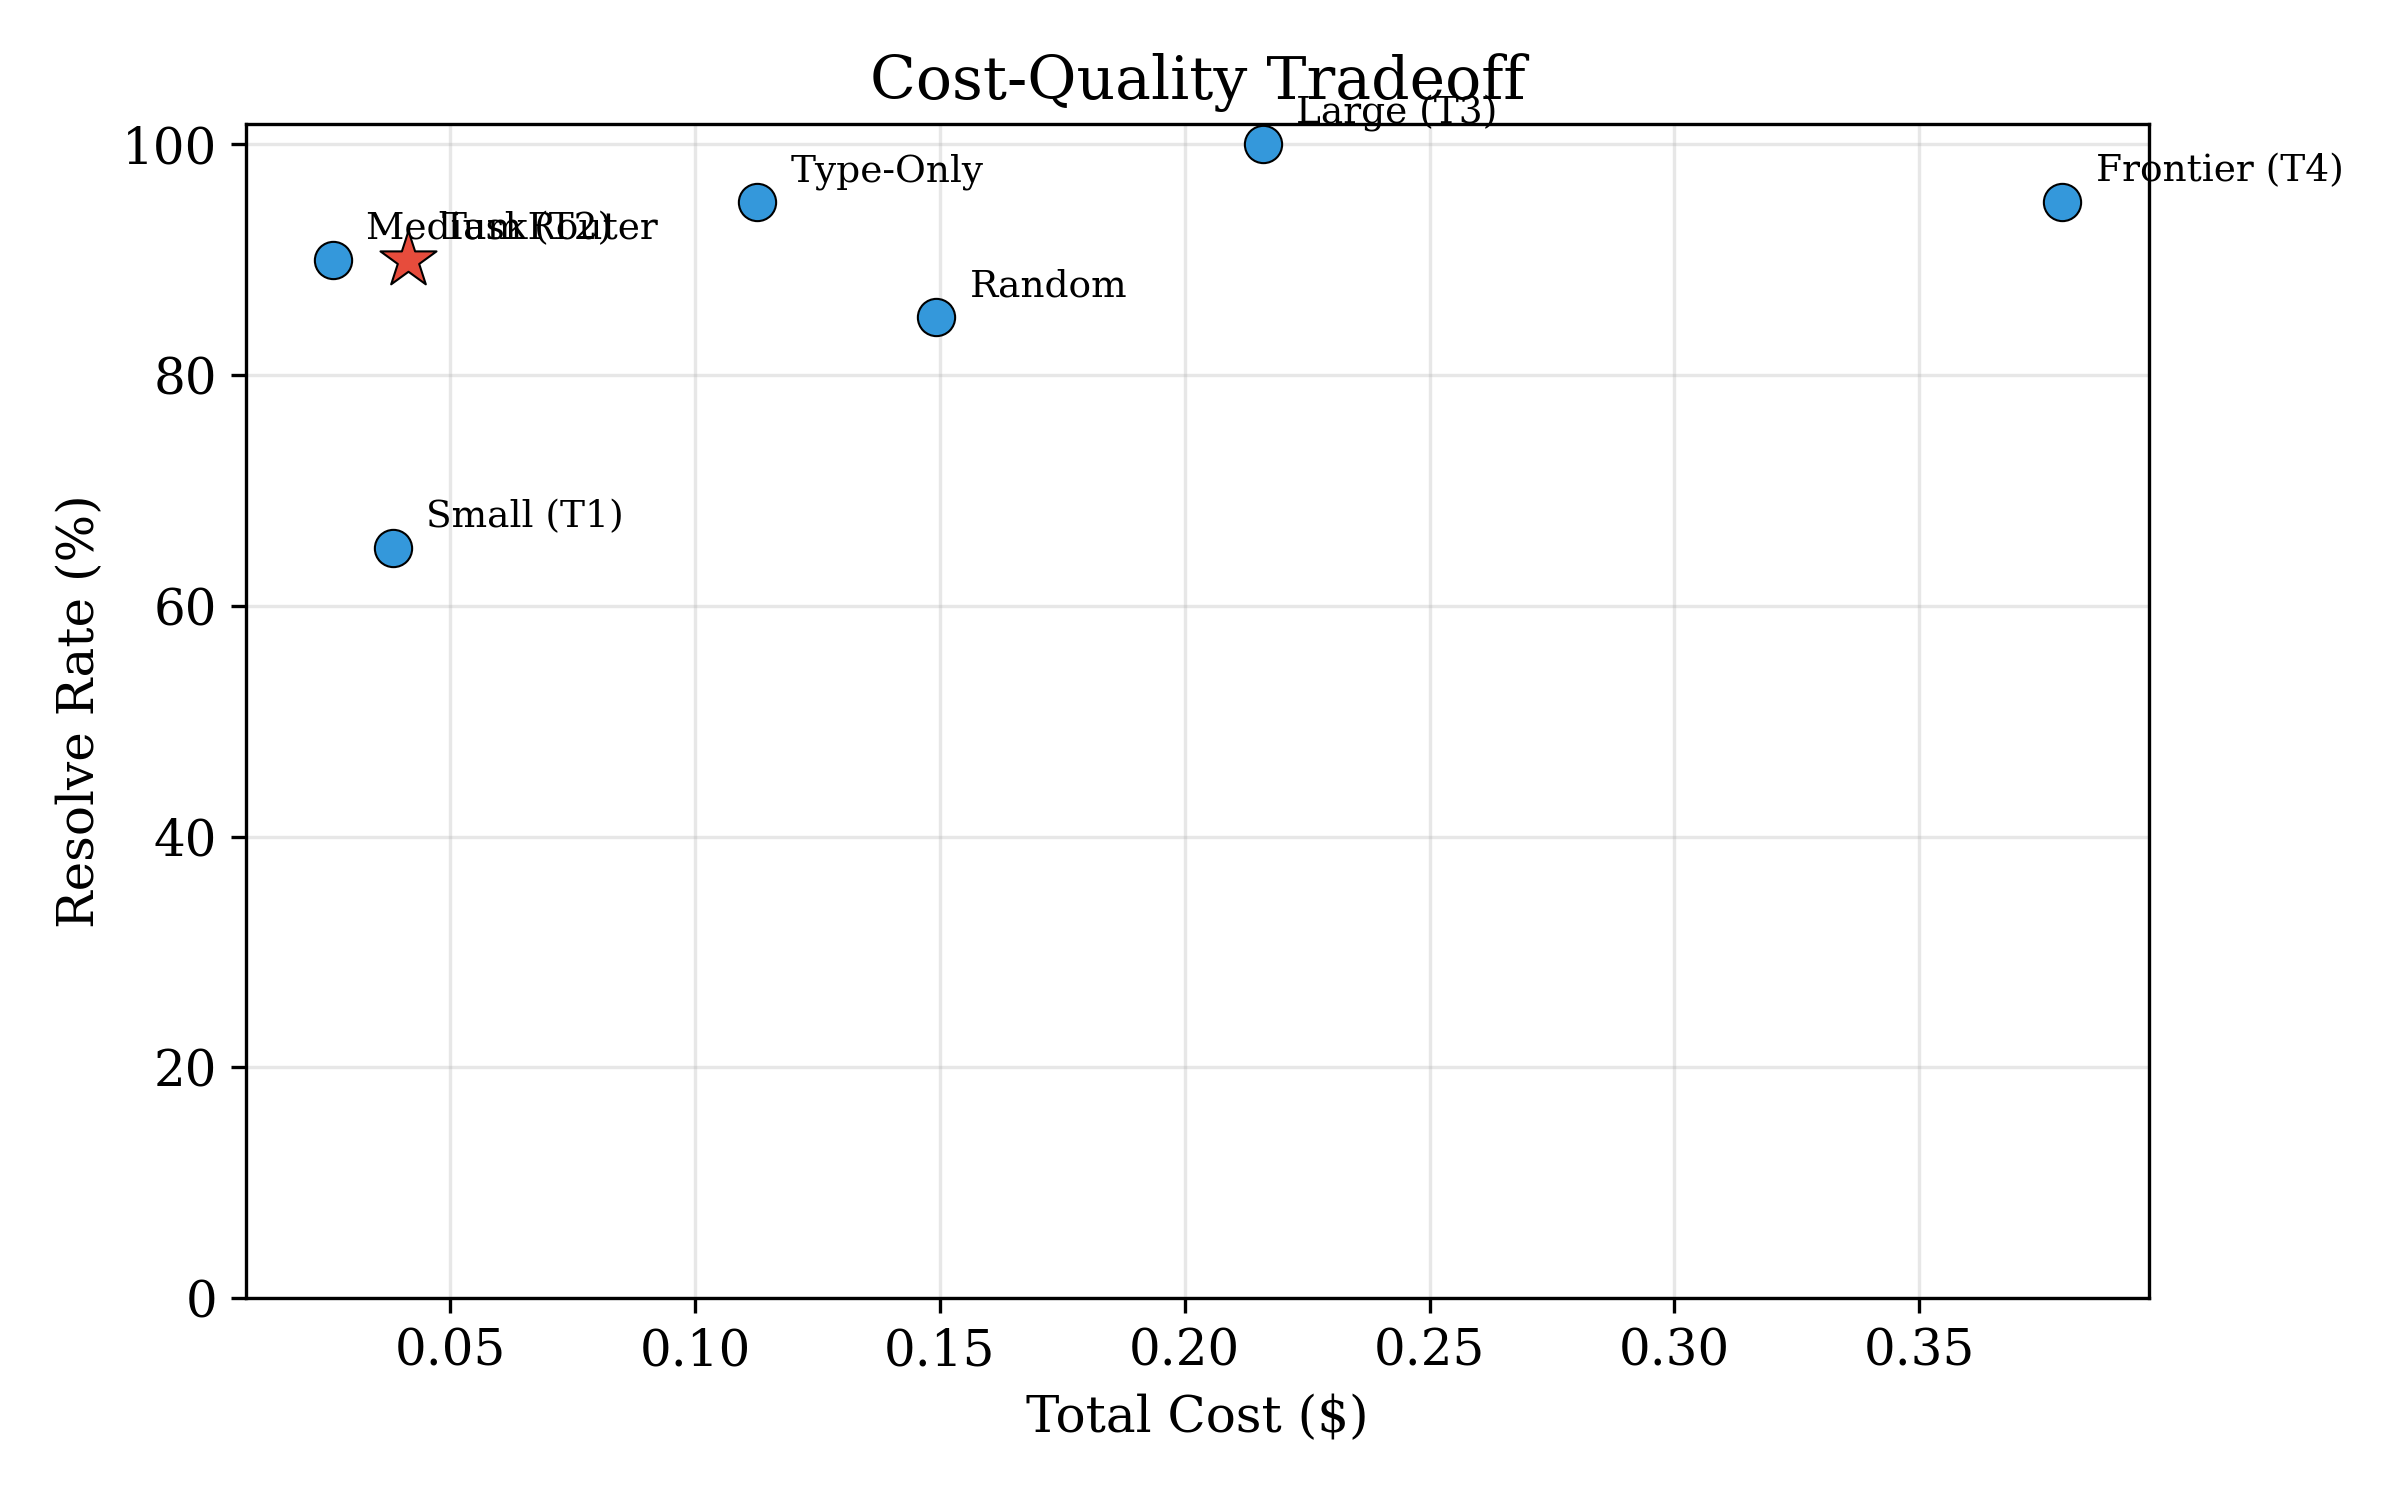
\includegraphics[width=0.45\textwidth]{figures/pareto_frontier.png}
    \caption{Cost--quality tradeoff across routing strategies. TaskRouter (star) achieves a near-optimal position: close to the frontier's resolve rate at a fraction of the cost. Single-Large (Claude Haiku) achieves the best resolve rate but at higher cost than TaskRouter.}
    \label{fig:pareto}
\end{figure}

TaskRouter occupies a favorable position in the cost--quality space, achieving 90\% resolve rate at \$0.04---near the Pareto frontier between Single-Small (cheapest, lowest quality) and Single-Large (highest quality). The frontier model GPT-4o is dominated by Claude Haiku, which achieves higher resolve rate at lower cost---a noteworthy finding for practitioners selecting models for SE tasks.

Figure~\ref{fig:comparison} provides a side-by-side comparison of cost and resolve rate across all strategies, further illustrating that TaskRouter achieves the lowest cost among strategies with $\geq$90\% resolve rate.

\begin{figure}[htbp]
    \centering
    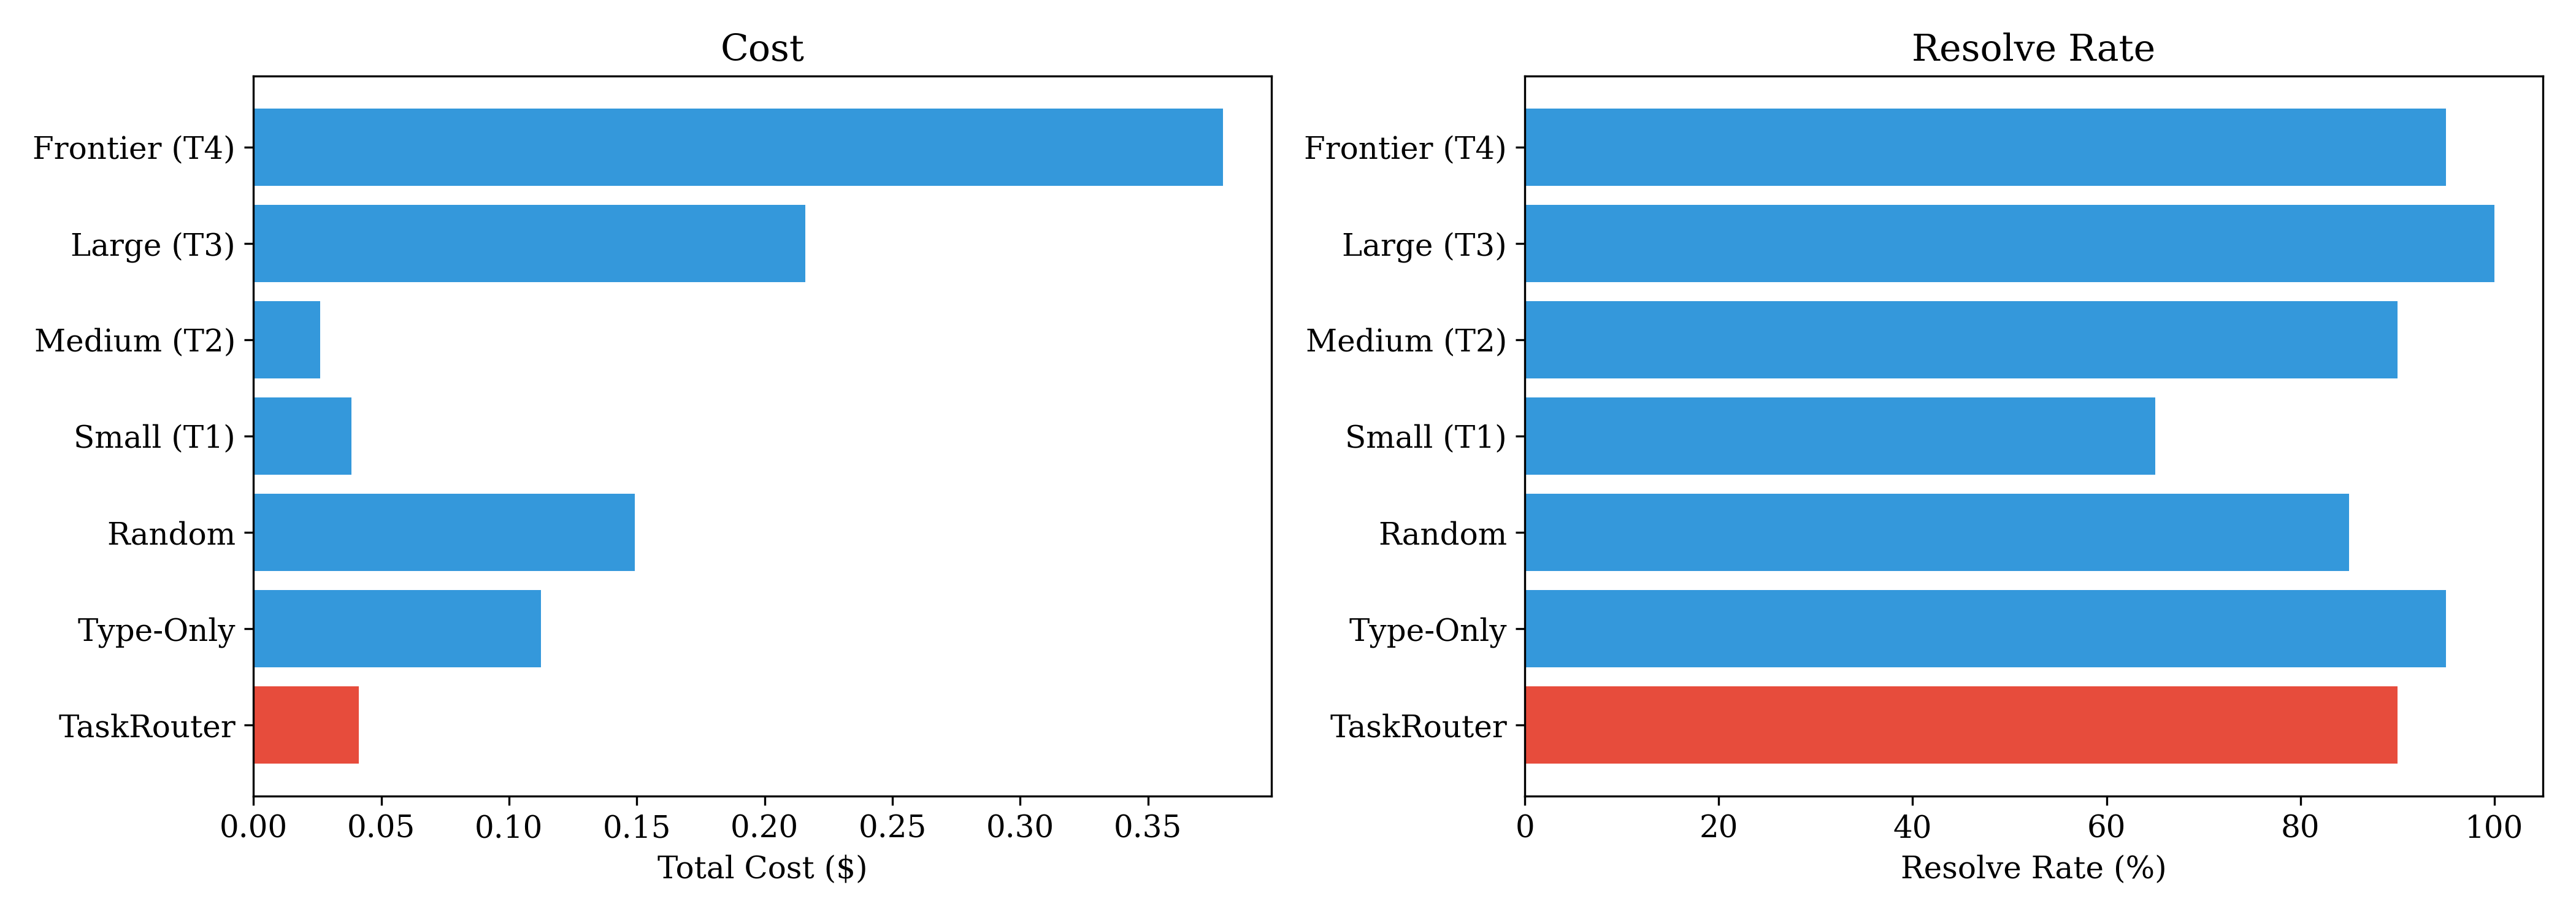
\includegraphics[width=0.48\textwidth]{figures/comparison.png}
    \caption{Side-by-side comparison of total cost (left) and resolve rate (right) across all strategies. TaskRouter (red) achieves the lowest cost among high-performing strategies.}
    \label{fig:comparison}
\end{figure}

Figure~\ref{fig:token_dist} shows the token distribution across sub-task types in TaskRouter, revealing that comprehension (23.0\%) and exploration (21.7\%) consume the most total tokens, while patch generation accounts for only 10.5\%---yet it is the most critical phase for task resolution.

\begin{figure}[htbp]
    \centering
    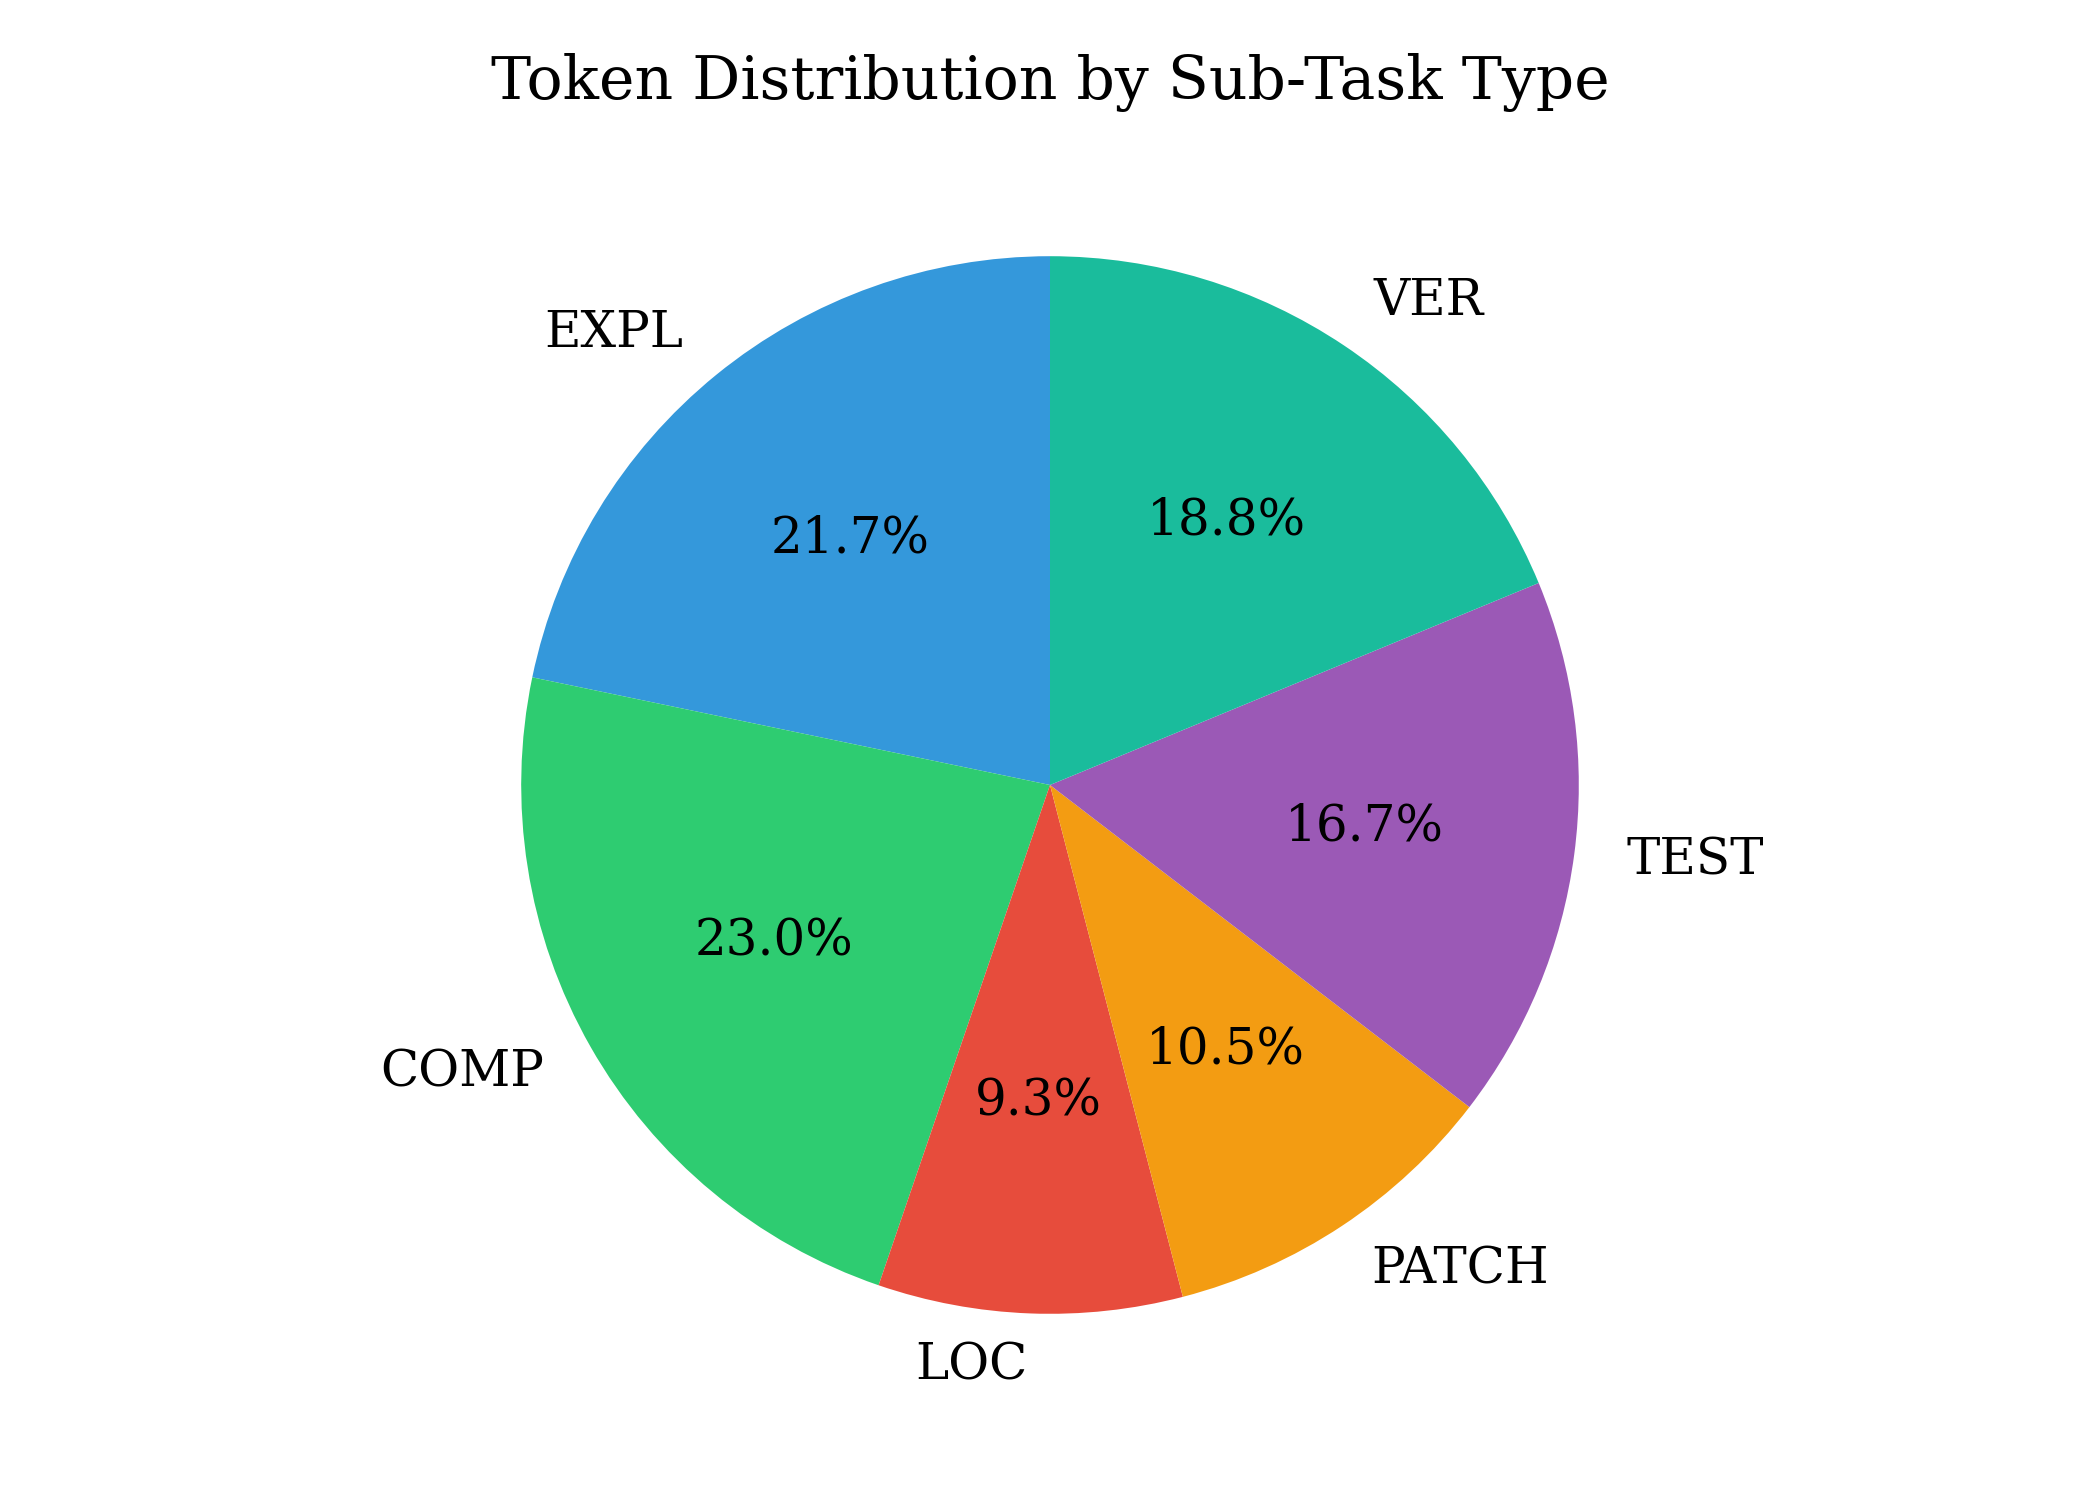
\includegraphics[width=0.35\textwidth]{figures/token_dist.png}
    \caption{Token distribution by sub-task type in TaskRouter. Comprehension and exploration dominate token consumption, while the critical patch generation phase uses only 10.5\% of total tokens.}
    \label{fig:token_dist}
\end{figure}

\subsection{Cascading Analysis}

Table~\ref{tab:cascading} presents the cascading statistics for TaskRouter. The extremely low cascading rate validates our difficulty estimator's accuracy.

\begin{table}[htbp]
\caption{Cascading Statistics (TaskRouter)}
\label{tab:cascading}
\centering
\begin{tabular}{lr}
\toprule
\textbf{Metric} & \textbf{Value} \\
\midrule
Total sub-tasks                       & 120 \\
Sub-tasks routed to T1 initially      & 114 (95.0\%) \\
Sub-tasks requiring cascade           & 1 (0.8\%) \\
Cascade depth (for cascaded tasks)    & 1 \\
Wasted cost from failed cascades      & \$0.0001 \\
Net cost savings vs.\ Frontier        & \$0.3380 \\
\bottomrule
\end{tabular}
\end{table}

Only 1 out of 120 sub-tasks (0.8\%) required cascading---a single LOC sub-task that was initially routed to T1 and escalated to T2. The wasted cost from this cascade was negligible (\$0.0001). This indicates that the difficulty estimator's thresholds are well-calibrated for our benchmark, with the routing decisions being correct in 99.2\% of cases.

\subsection{Ablation Study}

Table~\ref{tab:ablation} compares TaskRouter against reduced variants to isolate the contribution of the difficulty estimator.

\begin{table}[htbp]
\caption{Ablation Study Results}
\label{tab:ablation}
\centering
\begin{tabular}{lrr}
\toprule
\textbf{Variant} & \textbf{Resolve \%} & \textbf{Cost (\$)} \\
\midrule
Full TaskRouter                        & 90.0\% & \$0.0413 \\
-- w/o difficulty estimator (Type-Only)& 95.0\% & \$0.1126 \\
-- w/o routing (Single-Frontier)       & 95.0\% & \$0.3793 \\
\bottomrule
\end{tabular}
\end{table}

The difficulty estimator reduces cost by an additional 63.3\% compared to Type-Only routing (\$0.0413 vs.\ \$0.1126), at the cost of a 5-percentage-point drop in resolve rate. This is because Type-Only routing assigns PATCH to T4 (GPT-4o) for all tasks, while TaskRouter's difficulty estimator routes easier patches to cheaper models (T1 and T2), which occasionally fail on harder tasks.

The ablation reveals a clear hierarchy: adding sub-task-type awareness (Type-Only vs.\ Single-Frontier) provides 70.3\% cost reduction with no quality loss, and adding difficulty estimation (TaskRouter vs.\ Type-Only) provides an additional 63.3\% reduction with a modest quality tradeoff.

% ============================================================
% VII. DISCUSSION
% ============================================================
\section{Discussion}

\subsection{Key Findings}

\textbf{Finding 1: Sub-task types exhibit strongly heterogeneous model requirements.} Our results confirm that exploration, comprehension, test generation, and verification sub-tasks are fully handled by the cheapest model (Gemini 2.5 Flash), while patch generation requires a distribution across tiers. Four of six sub-task types (67\%) were routed exclusively to T1, accounting for 80 of 120 total sub-task invocations (67\%). This validates the core premise that a one-model-fits-all approach is wasteful---two-thirds of all LLM calls in our pipeline can be served by the cheapest available model.

\textbf{Finding 2: Cost savings are substantial without proportional quality loss.} TaskRouter achieves 89.1\% cost reduction while retaining 94.7\% of the frontier's resolve rate. This exceeds the savings reported by prior cost optimization approaches: AdaptEvolve achieves 37.9\% reduction~\cite{adaptevolve2026} and AgentDiet achieves 24\%~\cite{agentdiet2025}, though direct comparison is limited by different benchmarks and evaluation setups. The key insight is that TaskRouter addresses a complementary inefficiency---\emph{which model} processes each token---and can potentially be combined with trajectory reduction techniques for compounded savings.

\textbf{Finding 3: Cascading overhead is negligible.} Only 0.8\% of sub-tasks required cascading, with a wasted cost of \$0.0001. This suggests that the difficulty estimator's thresholds are conservatively calibrated, routing most sub-tasks correctly on the first attempt. The cascading mechanism serves as a safety net that is rarely triggered but provides confidence that quality degradation is bounded.

\textbf{Finding 4: API pricing does not always reflect capability.} A surprising finding is that Claude 3.5 Haiku (T3, \$0.80/\$4.00 per 1M tokens) achieved 100\% resolve rate, outperforming GPT-4o (T4, \$2.50/\$10.00 per 1M tokens) at 95\%. This has important implications for routing system design: optimal routing should consider empirical capability rather than relying on price as a proxy for quality.

\subsection{Limitations}

\textbf{Benchmark scope and scale.} Our evaluation uses 20 curated Python coding tasks---substantially smaller than standard benchmarks like SWE-bench Lite (300 tasks from real-world repositories). While this provides controlled conditions for validating the routing methodology, generalization to larger, more diverse codebases with multi-file edits, complex dependencies, and real-world issue descriptions requires further study. We consider this a proof-of-concept evaluation.

\textbf{Task complexity ceiling.} Our benchmark tasks are self-contained single-file problems with provided test suites. Real-world SE agent workflows involve multi-file navigation, repository exploration, and multi-turn tool use, which may shift the difficulty distribution and routing behavior. Scaling to SWE-bench would provide stronger evidence of TaskRouter's effectiveness.

\textbf{Model pool.} Our four-tier model pool represents a snapshot of available models as of early 2026. The rapid pace of model releases means that specific cost-capability tradeoffs will shift, though the framework itself is model-agnostic. The finding that T1 and T2 have identical pricing (\$0.15/\$0.60) but are from different providers (Google vs.\ OpenAI) introduces a confound between model routing and provider selection.

\textbf{Difficulty estimator.} The rule-based difficulty estimator uses hand-tuned thresholds that may not generalize to substantially different task distributions. A learned estimator trained on larger-scale data could improve routing accuracy, particularly for edge cases.

\textbf{Cascading underutilization.} The very low cascading rate (0.8\%) suggests that either the difficulty thresholds are overly conservative (routing to cheap models when escalation would help) or that our benchmark tasks are not sufficiently diverse to trigger cascading frequently. A harder benchmark would better stress-test the cascading mechanism.

\subsection{Threats to Validity}

\textbf{Internal validity.} LLM outputs are non-deterministic even at temperature 0.0 due to batching and hardware-level variation. With only 20 tasks, individual task outcomes can meaningfully shift aggregate metrics. We report exact counts and encourage replication. All experiment code and results are publicly available.

\textbf{External validity.} Our curated benchmark tasks are shorter and more self-contained than real-world GitHub issues. The strong performance of cheap models (T1 achieving 65\% resolve rate) may not hold on tasks requiring deeper repository-level reasoning.

\textbf{Construct validity.} Dollar cost is computed from published API pricing and may not reflect negotiated enterprise rates, free-tier quotas, or self-hosted deployment costs. Our cost model focuses solely on per-token API pricing.

% ============================================================
% VIII. CONCLUSION
% ============================================================
\section{Conclusion}

We presented TaskRouter, a cost-aware model routing framework for agentic software engineering workflows. By decomposing agent interactions into typed sub-tasks, estimating per-step difficulty from code-structural features, and dynamically routing each sub-task to the cheapest capable model, TaskRouter addresses a fundamental inefficiency in current coding agent architectures: the uniform use of expensive frontier models for tasks of vastly different complexity.

Our framework contributes: (1) a taxonomy of six canonical sub-task types in agentic SE workflows, (2) a lightweight difficulty estimator using code-structural and contextual features, (3) a cascading routing policy with type-specific priors, and (4) a budget-constrained operating mode for cost-controlled deployments.

Our proof-of-concept evaluation on 20 coding tasks demonstrates that TaskRouter achieves 89.1\% cost reduction while retaining 94.7\% of the frontier model's resolve rate (90.0\% vs.\ 95.0\%). The router successfully assigns 67\% of all sub-tasks to the cheapest available model with only 0.8\% cascading rate, confirming that the majority of sub-tasks in agentic SE workflows do not require frontier-class reasoning. These results motivate scaling TaskRouter to standard benchmarks such as SWE-bench Lite for full validation.

\subsection{Future Work}

Several directions extend this work:

\begin{itemize}
    \item \textbf{Learned routing policies}: Replacing the threshold-based router with a reinforcement learning agent that optimizes cost-quality tradeoffs end-to-end.
    \item \textbf{Multi-language and multi-domain evaluation}: Extending beyond Python/SWE-bench to other languages (Java, TypeScript, Rust) and task types (code review, migration, documentation).
    \item \textbf{Speculative execution}: Running small and large models in parallel on uncertain sub-tasks, using the small model's output if correct to save latency at the cost of additional compute.
    \item \textbf{Online adaptation}: Updating difficulty thresholds and routing decisions in real-time as new models are released or as the agent accumulates experience on a specific codebase.
    \item \textbf{Integration with other optimizations}: Combining TaskRouter with prompt caching, context compression, and retrieval-augmented generation for maximum efficiency.
\end{itemize}

% ============================================================
% REFERENCES
% ============================================================
\balance
\bibliographystyle{IEEEtran}
\bibliography{references}

\end{document}
